

On se doit de consid\'erer le cas o\`u dans le graphe de corr\'elation initial $G_C$, il existe des sommets $z$ tels que $Cliq(z) = -1$ et qu'aucun tel sommet $z$ n'est contenu dans une clique et qu'aucun de ses voisins n'est contenu par une clique.
Ce qui implique que tout sommet du graphe est dans la situation de $z$.

\begin{lemma}
Pour tout entier $n \ge 12$, il existe un graphe $G$ d'au moins $n$ sommets dans lequel aucun sommet n'est couvert par une ou deux cliques.
\end{lemma}

\begin{proof}
Ce lemme est tout d'abord bas\'e sur le fait que le graphe $G_0$ de la figure \ref{graphe_iourte_G0} le v\'erifie.
On obtient, \`a partir de $G_0$, un graphe avec $3$ sommets suppl\'ementaires v\'erifiant toujours cette propri\'et\'e en r\'ealisant la modification suivante. 
Ce graphe $G$ distingue trois sommets A, B, C. 
On remplace chaque ar\^ete $[A,B]$, $[B,C]$, $[A,C]$ par une chaine de longueur $2$.
Les sommets ainsi cr\'ees deviennent les nouveaux sommets distingu\'es A, B, C que l'on relie par un cycle de longueur $3$.
On peut ainsi propager cette modification autant de fois que n\'ecessaire pour atteindre $n$.
Ce qui cl\^ot la preuve du lemme.
\end{proof}

\begin{centering} \vspace{-0.5em}
\begin{figure}[htb!] \vspace{-0.5em}
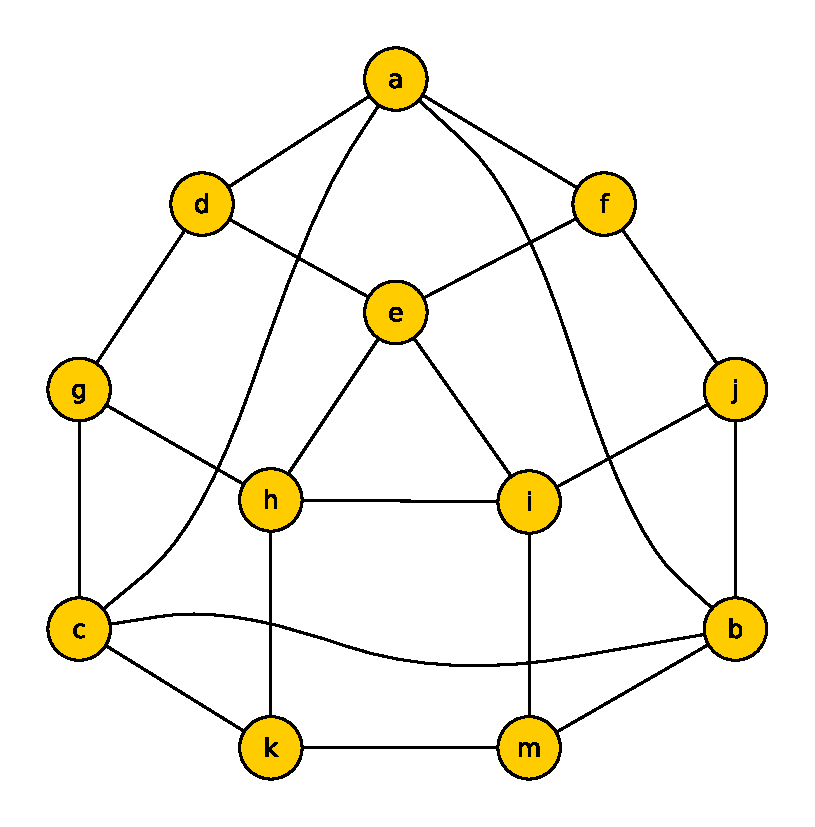
\includegraphics[scale=0.75]{grapheIourteG0.eps}
\caption{ Graphes $G_0$ o\`u aucun sommet n'est couvert par aucune clique }
\label{graphe_iourte_G0} 
\end{figure}
\end{centering} 

Notons $G_0^k$ avec $k \ge 1$ le graphe obtenu \`a partir de $k$ op\'erations de propagation \`a partir de $G_0$, graphe contenant donc $3k+12$ sommets, $6k+21$ ar\^etes et de degr\'e maximum \'egal \`a $4$.

\begin{theorem}
La distance-line de $G_0^k$ v\'erifie
$$ DL(G_0^k) \le 3k+6 $$
\end{theorem}

\begin{proof}
La figure \ref{graphe_iourte_G0_une_execution} d\'ecrit un line graphe $LG_0$ couvrant $G_0$ avec $6$ ar\^etes ne figurant pas dans $G_0$.
Le line graphe $LG_0^k$ couvrant et \`a distance $3k+6$ de $G_0^k$ est obtenu \`a partir  de $LG_0^{k-1}$ en supprimant une ar\^ete sur deux dans le cycle de taille $6$ form\'e par les anciens sommets $A$, $B$ et $C$ de $G_0^{k-1}$ et les nouveaux sommets $A$, $B$ et $C$ de $G_0^{k}$ (c'est-\`a-dire la suppression de $3$ ar\^etes).
Chaque ar\^ete restante sur ce cycle forme une nouvelle clique de taille $2$ et le nouveau cycle de taille $3$ entre $A$, $B$ et $C$  forme une nouvelle clique de taille $3$ (qui remplace la pr\'ec\'edente dans $LG_0^{k-1}$)....
\end{proof}

\begin{centering} \vspace{-0.5em}
\begin{figure}[htb!] \vspace{-0.5em}
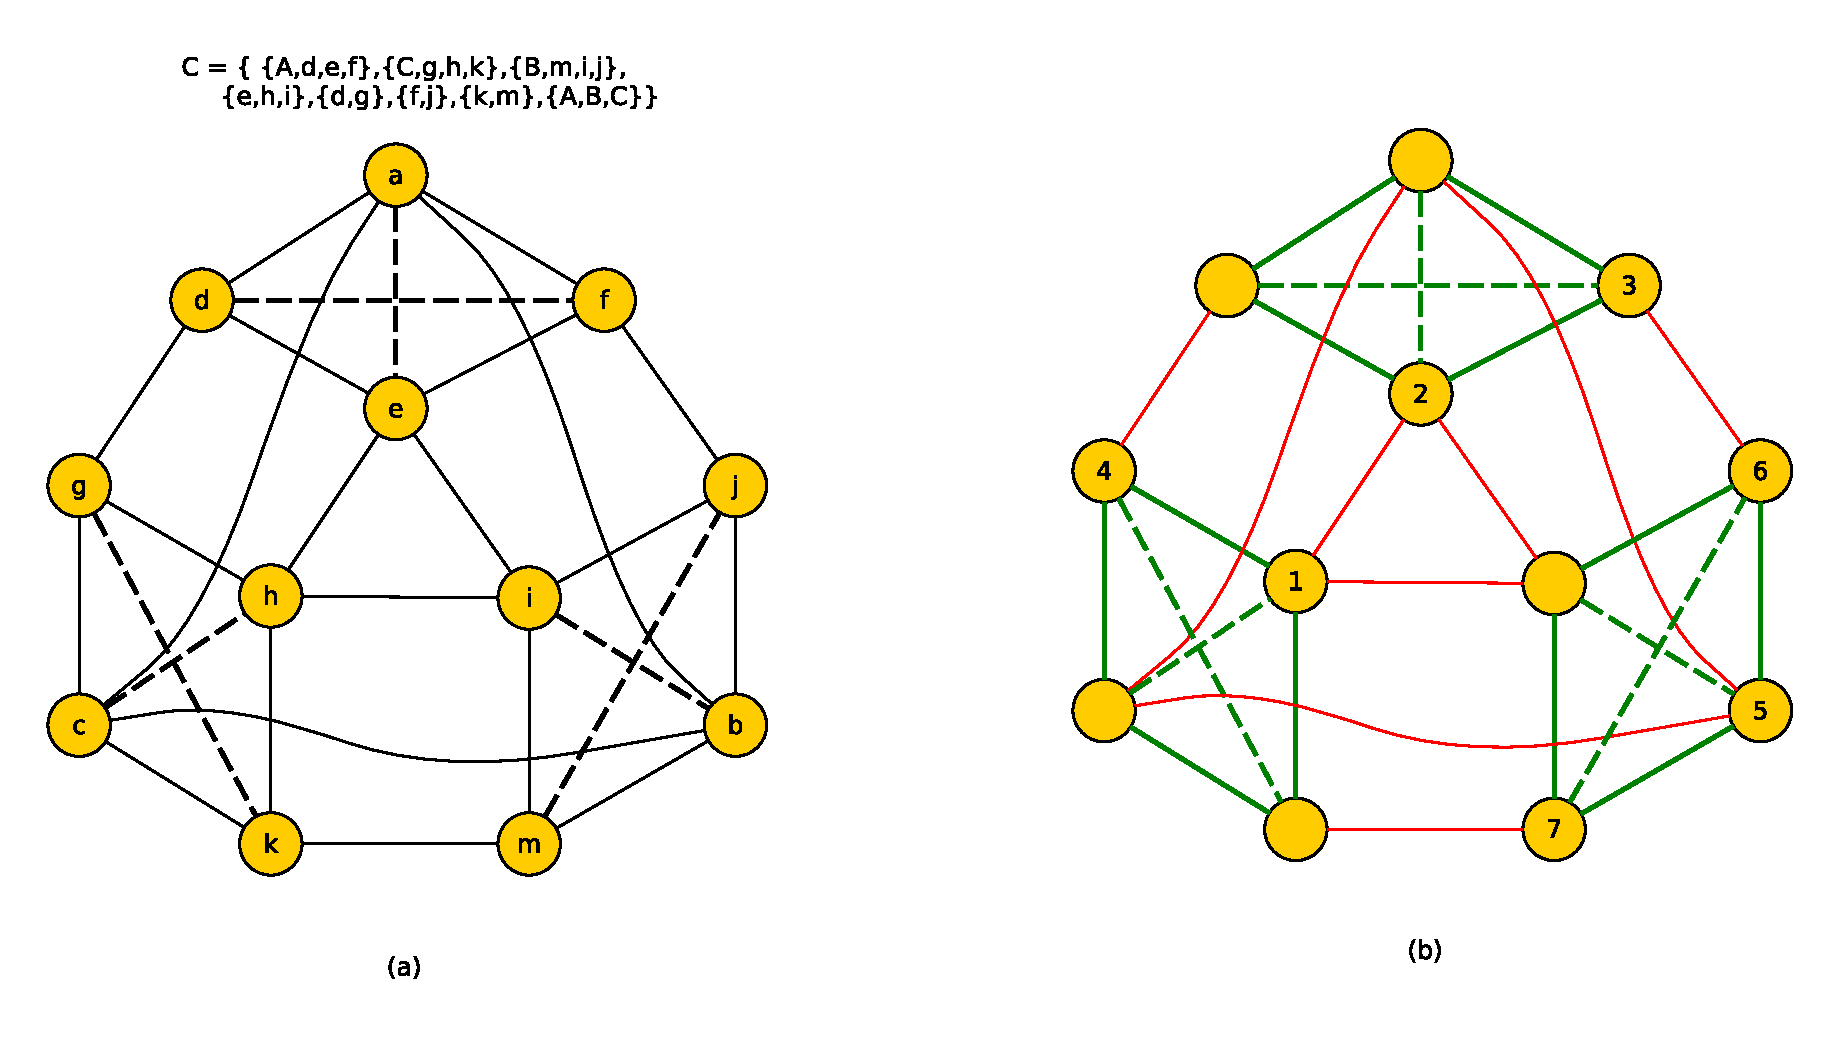
\includegraphics[scale=0.57]{grapheIourteG01eExecution.eps}
\caption{ (a) line graphe $LG_0$ \`a distance de Hamming $6$ de $G_0$ avec une couverture par cliques maximales $C$, et (b) une ex\'ecution (parmi celles possibles) de l'algorithme de compression transformant $G_0$ en $LG_0$}
\label{graphe_iourte_G0_une_execution} 
\end{figure}
\end{centering} 


